\documentclass[11pt]{article}
\usepackage[a4paper,margin=18mm]{geometry}
\usepackage[no-math]{fontspec}
\setmainfont{Latin Modern Roman}
\usepackage{amsmath,amssymb,amsthm,xfrac,xspace,hyperref,graphicx,comment}
\excludecomment{DefTralics}
\providecommand{\dpl}{\displaystyle}
\providecommand{\backmatter}{}
\providecommand{\loccit}{\emph{loc. cit.}}

\providecommand{\bibliofont}{\small}
\newcommand{\ie}{i.e.,\xspace}
\newcommand{\eg}{e.g.,\xspace}
\newcommand{\etc}{etc.\xspace}
\newcommand{\cf}{cf.\xspace}
\newcommand{\resp}{resp.\xspace}
\newcommand{\smaller}{\small}
\newcommand{\Subsection}{\subsection}
\newcommand{\Subsubsection}{\subsubsection}
\newcommand{\skpt}{\smallskip}
\emergencystretch=3em

% Begin literal retained input author-preamble.tex
\usepackage[scr=rsfs,cal=euler]{mathalfa}
\newcommand\mto{\mathchoice{\longmapsto}{\mapsto}{\mapsto}{\mapsto}}
\newcommand\hto{\mathrel{\lhook\joinrel\to}}

\usepackage{tikz, tikz-cd, pgfplots}
\usetikzlibrary{decorations.pathreplacing,calligraphy}
\usetikzlibrary{calc}

\tikzcdset{arrow style=Latin Modern}
\newcommand{\dradpl}{{\hspace*{-2mm}\begin{tikzcd}[ampersand replacement=\&,column sep = scriptsize]\mbox{}\ar[r,dashed]\&\mbox{}\end{tikzcd}\hspace*{-2mm}}}
\newcommand{\dratst}{{\hspace*{-2mm}\begin{tikzcd}[ampersand replacement=\&,column sep = small]\mbox{}\ar[r,dashed]\&\mbox{}\end{tikzcd}\hspace*{-2mm}}}
\let\drascst\dratst
\newcommand{\dra}{\mathchoice{\dradpl}{\dratst}{\drascst}{\drascst}}

\newcommand{\Psfrac}[2]{(\sfrac{#1}{#2})}
\newcommand{\psfrac}[2]{\sfrac{(#1)}{#2}}

\let\epsilon\varepsilon
\let\ts\textstyle

\theoremstyle{plain}
\newtheorem{theorem}{Theorem}[section]
\newtheorem{corollary}[theorem]{Corollary}
\newtheorem{lemma}[theorem]{Lemma}
\newtheorem{proposition}[theorem]{Proposition}
\newtheorem{Theorem}{Theorem}
\newtheorem{Conj}[Theorem]{Conjecture}
\renewcommand{\theTheorem}{\Alph{Theorem}}

\newtheorem*{corollary*}{Corollary}
\newtheorem*{question}{Question}

\theoremstyle{definition}
\newtheorem{remark}[theorem]{Remark}
\newtheorem{example}[theorem]{Example}
\newtheorem{definition}[theorem]{Definition}
\newtheorem*{remark*}{Remark}
\newtheorem*{Fact}{Fact}


\renewcommand\AA{{\mathbb A}}
\newcommand\CC{{\mathbb C}}
\newcommand\FF{{\mathbb F}}
\newcommand\NN{{\mathbb N}}
\newcommand\PP{{\mathbb{P}}}
\newcommand\QQ{{\mathbb Q}}
\newcommand\ZZ{{\mathbb Z}}

\newcommand\Cc{{\mathcal C}}
\newcommand\Lc{{\mathcal L}}
\newcommand\Oc{{\mathcal O}}
\newcommand\Qc{{\mathcal Q}}

\newcommand\Cl{{\mathrm{Cl}}}
\newcommand\cond{{\mathrm{cond}}}
\newcommand\tdiv{{\mathrm{div}}}
\newcommand\Ext{{\mathrm{Ext}}}
\newcommand\Hom{{\mathrm{Hom}}}
\newcommand\lct{\mathrm{lct}}
\newcommand\length{{\mathrm{length}}}
\newcommand\loc{{\mathrm{loc}}}
\newcommand\norm{{\mathrm{norm}}}
\newcommand\Pic{{\mathrm{Pic}}}
\newcommand\red{{\mathrm{red}}}
\newcommand\Spec{{\mathrm{Spec}}}
\newcommand\wt{{\mathrm{wt}}}

\newcommand\Dcy{{D^{\mathrm{CY}}}}
\newcommand\Dss{{D^{\mathrm{ss}}}}
\newcommand\Dsso{{D^{\mathrm{ss}}_0}}
\newcommand\Dcyo{{D^{\mathrm{CY}}_0}}
\newcommand\Dnorm{{D^{\mathrm{norm}}}}
\newcommand\Dnormo{{(\Dnorm)_0}}
\newcommand\Do{{D_0}}
\newcommand\Xcy{{X^{\mathrm{CY}}}}
\newcommand\Xcyo{{X^{\mathrm{CY}}_0}}

\newcommand\Yt{{\widetilde{Y}}}
\newcommand\Ct{{\widetilde{C}}}
\newcommand\St{{\widetilde{S}}}

\newcommand\cl{{\colon}}
\newcommand\Pabc{{\PP(a^2,b^2,c^2)}}
\newcommand\xbar{{\bar{x}}}
\newcommand\ybar{{\bar{y}}}

\let\hra\hto

\definecolor{greener}{RGB}{72,171,131}

\pgfplotsset{compat=1.18}

% End literal retained input author-preamble.tex

\begin{document}
\begin{center}{\Large Stable item 2247}\end{center}
\paragraph{Source and attribution.}
Kristin DeVleming, David Stapleton, \emph{Smooth limits of plane curves of prime degree and Markov numbers}, Journal de l’École polytechnique — Mathématiques 11 (2024), publisher version, DOI 10.5802/jep.263. \href{https://jep.centre-mersenne.org/articles/10.5802/jep.263/}{Publisher article}. Authors' text: \href{https://creativecommons.org/licenses/by/4.0/}{CC BY 4.0}.
\paragraph{Editorial problem boundary.}
Prove only Theorem1.10 below: for a nontrivial Markov triple in the printed nondecreasing order, every degree greater than2 that is a multiple of its largest entry admits a smooth projective nonplanar limit of complex plane curves. Preserve the separate c equals2 case, the precise Manetti partial smoothings, divisor-class and intersection conventions, smooth-divisor deformation and gonality-pencil argument. The complete new required divisor-extension, class/Picard, base-point and section-lifting proofs are retained. Broader conjectures and the quintic/septic casework are unselected. The original Markov-tree illustration remains an exact vector asset.
\paragraph{Difficulty (editorial): H3.}
Knowing that a weighted projective plane smooths to the plane does not extend the needed divisor class or guarantee a smooth member of its linear system on the partial smoothing. The authors control extension obstructions, compute the class/Picard and intersection scaling, and prove global generation and cohomology constancy for the relevant divisorial sheaves. Those new deformation and section-lifting results construct the smooth limit and its low-degree pencil before the standard gonality comparison, beyond merely applying the known Manetti surface classification.
\paragraph{Editorial transcription note.}
Original author language, mathematics and ordering are preserved. Publisher front matter is replaced by this independent article wrapper. Bibliography is recovered from matching cached publisher HTML, including its TeX formulas. No new proof or mathematical repair is supplied. Surrounding original results are retained for conservative context and are not extra selected corpus claims.
\clearpage

% Begin literal retained input original-summary-statement.tex
\begin{Theorem}\label{thmA:nonplanarlimits}
For any Markov number $d >2$, there is family of smooth plane curves of degree $d$ with a smooth projective non-planar limit. In particular, for any Markov number $p>2$ that is prime there is a smooth family of prime degree $p$ plane curves with a non-planar central fiber.
\end{Theorem}

% End literal retained input original-summary-statement.tex


% Begin literal retained input author-body.tex
\section{Markov numbers and degenerations of the projective plane}\label{sec:degensofP2}

The goal of this section is to prove Theorem \ref{thmA:nonplanarlimits}, \ie to show that for any Markov number $d$ there is a smooth limit of degree $d$ curves that is not planar. These limits are constructed as Cartier divisors in degenerations of the plane with isolated singularities. In the process we study some of the basic properties of the log terminal $\QQ$-Gorenstein degenerations of $\PP^2$; \eg we compute their Class groups and show that any ample line bundle is globally generated. To show these divisors are not planar we give an upper bound on their gonality that is less than $d-1$, the gonality of a smooth degree~$d$ plane curve.

We start by considering weighted projective planes that are limits of $\PP^2$. To start we show how the Markov equation arises when considering these weighted projective spaces. Suppose there is a flat family
\[
X \to T
\]
over a pointed curve $0\in T$ such that $X$ is $\QQ$-Gorenstein and for $t\in T$ general $X_t\cong \PP^2$ and $X_0\cong \PP(p,q,r)$ is a weighted projective plane (with $p$, $q$, and $r$ coprime). Then in fact, $(p,q,r)=(a^2,b^2,c^2)$ and $(a,b,c)$ satisfy:
\begin{flalign*}
\text{(the Markov equation)}&&a^2+b^2+c^2=3abc.&&\phantom{\text{(Markov Equation)}}
\end{flalign*}
All solutions to the Markov equation are obtained by successively permuting or performing the \textit{mutation} $(a,b,c) \mto (a,b,3ab - c)$ starting from the minimal solution $(1,1,1)$ \cite{Markov, Mutations}. The first few triples in the Markov tree are
\begin{center}
\scalebox{1.2}{
% Begin literal retained input devleming-stapleton_figures/markovtree.tex
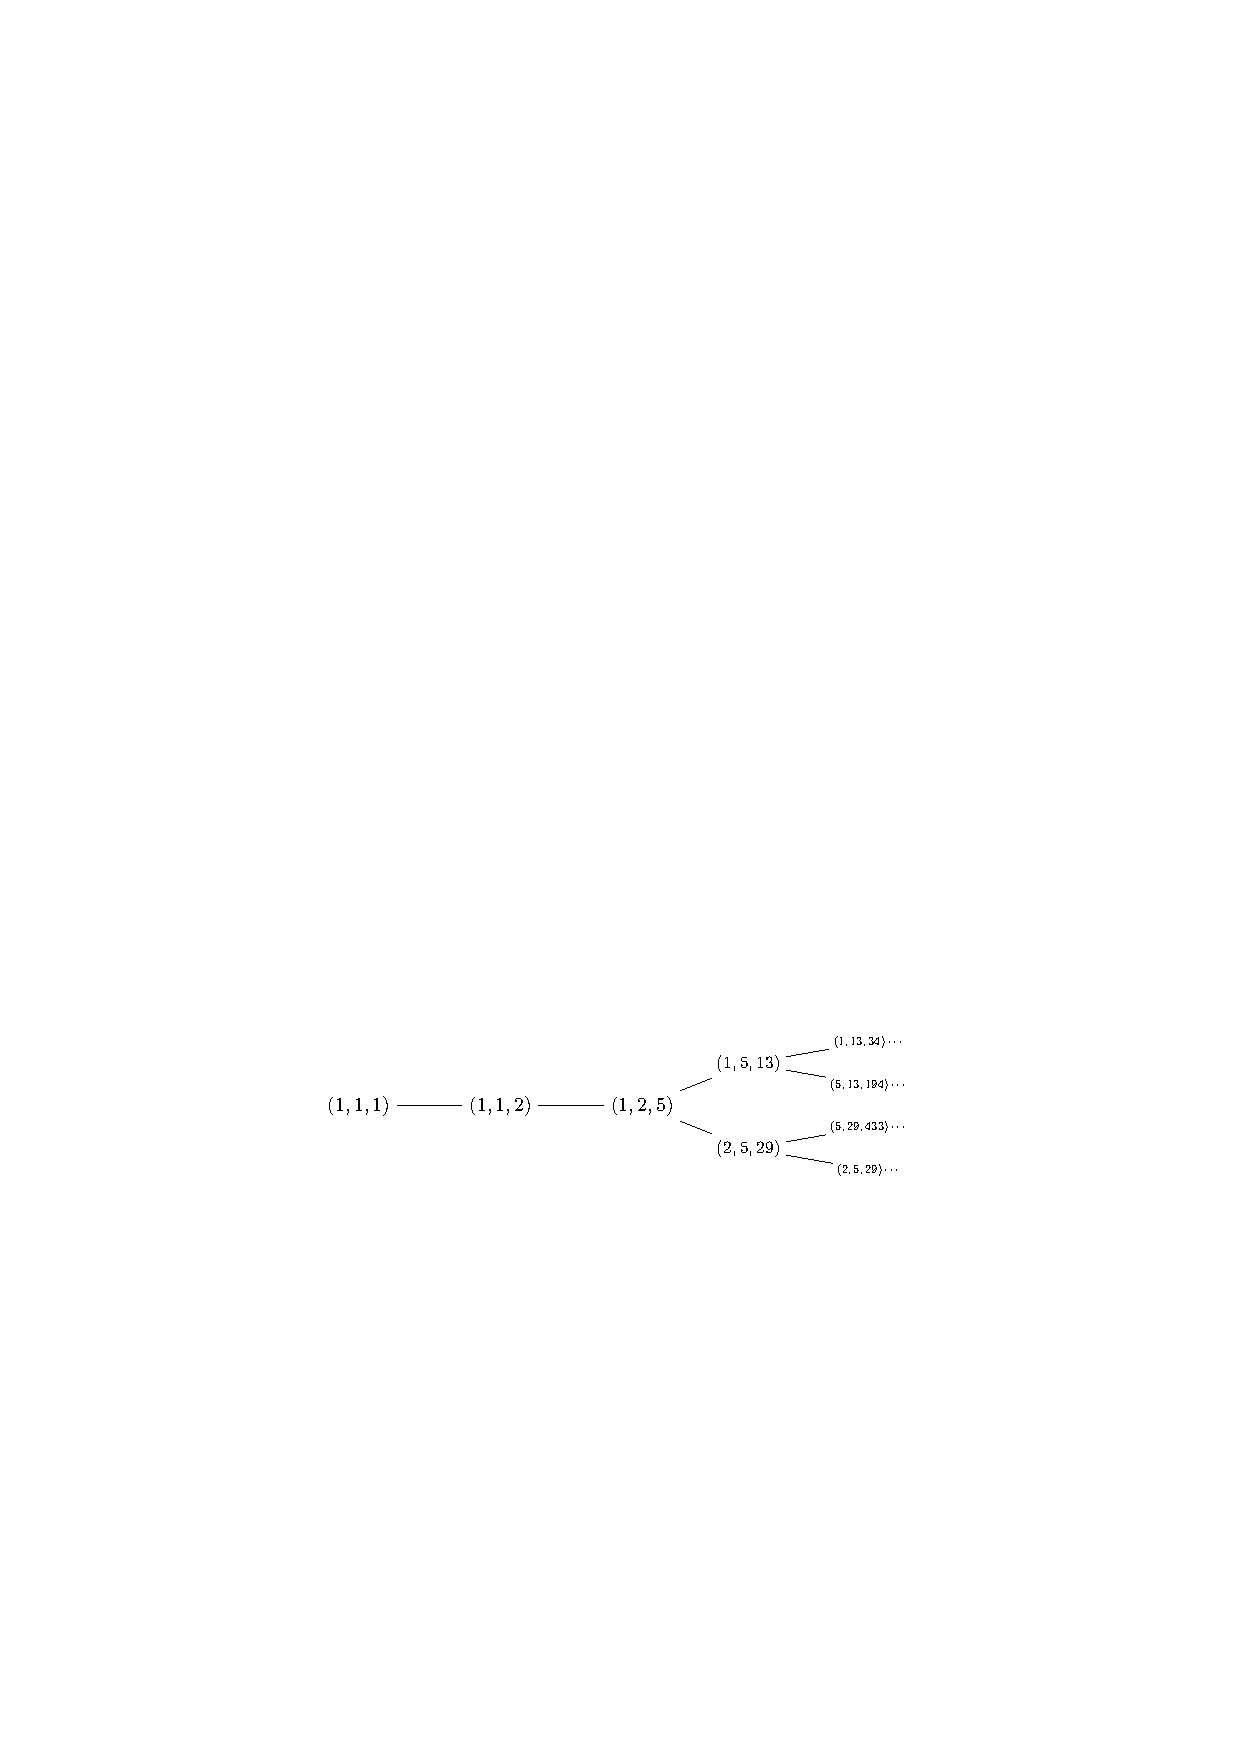
\includegraphics[width=237.5pt]{../assets/2247/devleming-stapleton_figures/markovtree-original-vector.pdf}

% End literal retained input devleming-stapleton_figures/markovtree.tex
}
\end{center}
corresponding to the weighted projective spaces $\PP^2$, $\PP(1,1,4)$, $\PP(1,4,25),\dots$.

The fact that Markov numbers show up when considering $\QQ$-Gorenstein degenerations of $\PP^2$ is a consequence of the constancy of the anticanonical volume $(-K_{X_t})^2$ (Kollár addresses the top self-intersection of a $\QQ$-Cartier divisor $D$ over $T$ in much more generality in \cite[Th.\,11]{KollarConstantVolume}). Setting the anticanonical volume of $\PP(p,q,r)$ equal to $(-K_{\PP^2})^2 = 9$ gives
\[
(p+q+r)^2/pqr = 9.
\]
So $(p+q+r) = 3\sqrt{pqr}$. As $p$, $q$, and $r$ are all coprime, the only possibility is they are all perfect squares. In fact, one can show that for any Markov triple $(a,b,c)$ the singularities of the weighted projective space $\PP(a^2,b^2,c^2)$ can be independently smoothed in a $\QQ$-Gorenstein family which implies that every such weighted projective space is a limit of $\PP^2$ \cite[Cor.\,1.2]{HackProk}. These surfaces were first studied by Manetti in~\cite{Manetti} and are called Manetti surfaces.

\begin{definition}[Manetti surfaces]
Fix a Markov triple $(a,b,c)$. Define
\[
M(a,b,c):= \PP(a^2,b^2,c^2).
\]
Define $M(b,c)$ to be the partial smoothing of the index $a^2$ singularity in $M(a,b,c)$ --- \ie $M(b,c)$ has 2 singularities of index $b^2$ and $c^2$. Likewise define $M(c)$ to be the smoothing of the index $a^2$ and $b^2$ singularities in $M(a,b,c)$.
\end{definition}

\begin{remark}
The singularities appearing on Manetti surfaces are examples of $T$ singularities. In the notation of Hacking and Prokhorov, they are $T_1$ singularities, and the versal $\QQ$-Gorenstein deformation space of such a singularity is one-dimensional (\cf \cite[p.\,4]{HackProk}), so any non-trivial deformation of such a singular point smooths it completely. Throughout this section, we will therefore use the terminology \textit{partial smoothing} of a Manetti surface $M_0$ to mean a one parameter flat family $M$ over a smooth pointed curve $0\in T$ such that $M$ has $\QQ$-Gorenstein singularities, $M_0$ is the fiber over $0 \in T$, and for any singular point in $M_0$ the local deformation of the singularity is either a smoothing or a trivial deformation.
\end{remark}

% End literal retained input author-body.tex

\stepcounter{theorem}

% Begin literal retained input additional-author-body.tex
In fact, Hacking and Prokhorov prove that \textit{every} log terminal $\QQ$-Gorenstein degeneration of $\PP^2$ is a Manetti surface.

\begin{theorem}[{\cite[Cor.\,1.2]{HackProk}}]\label{thm:manettisurfaces}
The log-terminal $\QQ$-Gorenstein degenerations of $\PP^2$ are precisely the Manetti surfaces.
\end{theorem}

Let $M$ be a partial smoothing of a Manetti surface $M_0$ over a smooth pointed curve. If $M_t$ is a general fiber of $M$, we say a divisorial sheaf $\Oc_{M_0}(D_0)$ on $M_0$ \textit{extends to $M_t$} if there is a divisorial sheaf $\Oc_{M}(D')$ on $M$ such that $\Oc_{M}(D')|_{M_0} \cong \Oc_{M_0}(D_0)$. We call $\Oc_{M}(D')|_{M_t}$ the \textit{extension} of $\Oc_{M_0}(D_0)$ to $M_t$. The next lemma shows that any divisorial sheaf on $M_0$ that is Cartier at the smoothed singularities extends to~$M_t$. A~priori, such an extension is not unique, but once we prove that any Manetti surface has class group $\ZZ$ and that the intersection numbers are preserved in partial smoothings, it follows that the extensions are unique.

\begin{lemma}\label{extendingdivisors}
Let $M_0$ be a del Pezzo surface (a normal, log terminal surface with ample anticanonical divisor), and let $M$ be a $1$-parameter $\QQ$-Gorenstein partial smoothing of $M_0$. If $\Oc(D_0)$ is a divisorial sheaf on $M_0$ that is locally free at any partially smoothed singularities then there is a base change $T'\to T$ such that $\Oc(D_0)$ extends to a divisorial sheaf on $M \times_T T'$.
\end{lemma}

\begin{proof}
We show that the obstruction to extending $\Oc_{M_0}(D_0)$ vanishes. Assume $\Oc(D_0)$ extends to a divisorial sheaf $\Oc(D_{0,n})$ on an infinitesimal deformation $M_n$ of $M_0$ over $\CC[t]/t^n$. The obstruction to extending $\Oc(D_{0,n})$ to a divisorial sheaf on $M_{n+1}$ over $\CC[t]/t^{n+1}$ is a class in
\[
\Ext^2_{\Oc_{M_n}}(\Oc_{M_n}(D_{0,n}),\Oc_{M_0}(D_0))
\]
(see \eg \cite[\href{https://stacks.math.columbia.edu/tag/08L8}{Tag 0ECH}]{stacks-project}). The local-to-global spectral sequence shows that all the obstructions are local and supported at the non-smoothed points: \[H^2(M_n,\mathcal{H}\mathrm{om}(\Oc(D_{0,n}),\Oc(D_0))) = H^2(M_0,\Oc_{M_0}) = 0\] by Kodaira vanishing, and $\mathcal{E}\mathrm{xt}^1(\Oc(D_{0,n}),\Oc(D_0))$ is supported on the non-smoothed points). So the obstruction lives in
\[
H^0(M_n,\mathcal{E}\mathrm{xt}^2(\Oc(D_{0,n}),\Oc(D_0))).
\]
This shows the obstructions are local and supported at the non-smoothed point. But locally at this point, the deformation of $M_0$ is trivial, thus there is no local obstruction and $\Oc(D_{0,n})$ extends. Lastly, it may be necessary a priori to make a base change $T'\to T$ to make the above deformation algebraic.
\end{proof}

\begin{theorem}\label{thm:classpicofmanettisurfaces} Let $M_0$ be a $\QQ$-Gorenstein degeneration of $\PP^2$.
\begin{enumerate}
\item\label{thm:classpicofmanettisurfaces1}
$\Cl(M_0)=\ZZ$ and $\Pic(M_0)=\ZZ$. We write $\Oc_{M_0}(1)$ for the positive generator of $\Cl(M_0)$.
\item\label{thm:classpicofmanettisurfaces2}
If $A$ is the direct sum of the local class groups at the singular points of $M_0$, then the sequence:
\[
0\to \Pic(M_0)\to \Cl(M_0)\to A\to 0
\]
is exact. In particular, the map from $\Pic(M_0)$ to $\Cl(M_0)$ is multiplication by $\alpha^2=|A|$.
\item\label{thm:classpicofmanettisurfaces3}
With the notation from \eqref{thm:classpicofmanettisurfaces2}, $\Oc_{M_0}(1)$ has self intersection number $1/\alpha^2$.
\item\label{thm:classpicofmanettisurfaces4}
Let $M \to T$ be a $1$-parameter $\QQ$-Gorenstein partial smoothing of $M_0$. Let $B$ be the local class group of the smoothed singularities and let $\beta=\sqrt{|B|}\in \ZZ$. A divisor $D_0\in \Cl(M_0)$ extends to a divisor $D = D_{T'}$ on $M \times_T T'$ for a base change $T' \to T$ if and only if $\Oc_{M_0}(D_0) = \Oc_{M_0}(m \beta)$ for some integer $m$. Furthermore, over a general point, the extension $D$ is in $|\Oc_{M_t}(m)|$.
\item\label{thm:classpicofmanettisurfaces5}
If $D$, $D'$ are two $\QQ$-Cartier Weil divisors on $M$ then the intersection numbers $(D|_{M_t})\cdot (D'|_{M_t})$ are independent of $t\in T$.
\end{enumerate}
\end{theorem}

\begin{proof}
We know that $M_0$ is a partial smoothing of a weighted projective space $\PP:=\Pabc$. For weighted projective spaces the map from the class group to the local class groups is surjective. Thus it follows from Lemma \ref{extendingdivisors} that the map
\[
\Cl(M_0)\to A
\]
is surjective, which shows the sequence in (2) is exact.

The divisor $\Oc(-K_{\PP})=\Oc_{\PP}(3abc)$ extends to the divisor $K_{M_0}$ on $M_0$. Let $B$ (\resp $A$) be the local class group of the smoothed (\resp unsmoothed) singularities. By Lemma~\ref{extendingdivisors}, $\Oc_\PP(|B|)$ extends to $M_0$. Set $\beta = \sqrt{|B|}$, so $\beta=\mathrm{gcd}(|B|, 3abc$), and set $\alpha=\sqrt{|A|}$. Then $\Oc_\PP(\beta)$ extends to a divisorial sheaf $\Oc_{M_0}(1)$ on $M_0$, and $\Oc_{M_0}(1)$ generates the local class group of the unsmoothed singularities. Now we wish to prove that $\Oc_{M_0}(1)$ generates $\Cl(M_0)$.

It is known that $\Pic(M_0)=\ZZ$ (\cite[Lem.\,2.1, Prop.\,6.3]{Hacking}). Let $\Oc_{M_0}(1)\in \Cl(M_0)$ be the divisor on $M_0$ from the previous paragraph (\ie $\Oc_\PP(\beta)$ extends to $\Oc_{M_0}(1)$ on~$M_0$). We will show that $\Oc_{M_0}(1)$ generates $\Cl(M_0)$. Consider the following diagram:\vspace*{-3pt}
\[
\begin{tikzcd}
0\arrow[r] & \ZZ\cdot \Oc_{M_0}(\alpha^2)\arrow[r] \arrow[d]& \ZZ\cdot \Oc_{M_0}(1)\arrow[r]\arrow[d] & \ZZ/\alpha^2\ZZ\arrow[r]\arrow[d] &0\\
0 \arrow[r] &\Pic(M_0)\arrow[r] & \Cl(M_0)\arrow[r] & A\arrow[r] &0.
\end{tikzcd}
\]
It suffices to show that the map $\ZZ\cdot \Oc(\alpha^2)$ to $\Pic(M_0)$ is surjective.

As $K_{M_t}^2$ is constant in the family $M \to T$ and the restriction of every divisor $D|_{M_t}$ is numerically a rational multiple of $K_{M_t}$, the intersection numbers of divisors are constant in the family (proving \eqref{thm:classpicofmanettisurfaces5}). On the central fiber, if $D_0 \in |\Oc_\PP(\beta)|$, then $D_0^2 = \sfrac{\beta^2}{\alpha^2\beta^2} = \sfrac{1}{\alpha^2}$. Therefore, $\Oc_{M_0}(1)^2 = \sfrac{1}{\alpha^2}$ (proving \eqref{thm:classpicofmanettisurfaces3}).

Now, let $\Lc$ be the ample generator of $\Pic(M_0)$. Then $\Lc \equiv_{\mathrm{num}} \Oc_{M_0}(\mu)$ so $\Oc_{M_0}(\mu)\cdot \Oc_{M_0}(1)$ is an integer. Let $D_0 \in |\Oc_{M_0}(1)|$. As $\alpha^2D_0$ is Cartier, $\mu \le \alpha^2$. Therefore, because $\Oc_{M_0}(\mu)\cdot \Oc_{M_0}(1) = \mu \cdot\sfrac{1}{\alpha^2}$, we must have $\mu = \alpha^2$. This implies that $\Lc = \Oc(\alpha^2 D_0) $ and $\Oc(\alpha^2 D_0)$ generates $\Pic(M_0)$. This completes the proof of \eqref{thm:classpicofmanettisurfaces1}.

To prove \eqref{thm:classpicofmanettisurfaces4}, assume that (after possibly base changing) that $\Oc_{M_0}(\mu)$ extends to an ample generator $\Oc_{M_t}(1)$ of $\Cl(M_t)$ for a general fiber $M_t$ of $M$.
As~$H^1(M_0, \Oc_{M_0}(D_0)) = 0$, the divisor $D_0$ then extends to a divisor $D$ on $M$. By \eqref{thm:classpicofmanettisurfaces5} we have $\Oc_{M_0}(\mu)^2 = \Oc_{M_t}(1)^2$. By \eqref{thm:classpicofmanettisurfaces3} the left hand side is $\mu^2/\alpha^2$ (where $\alpha^2 = |A|$, where~$A$ is the local class group of the singularities of $M_0$). And by \eqref{thm:classpicofmanettisurfaces3} the right hand side is $\beta^2/\alpha^2$ which proves that $\Oc_{M_0}(\mu)$ extends to a divisorial sheaf on $M$ if and only if $\mu = \beta$.
\end{proof}

We thank János Kollár for suggesting improvements to the following results in this section.

\begin{theorem}\label{thm:curveinsmoothlocusdP}
Let $X_T\to T$ be a flat projective family over a smooth pointed curve $0\in T$. Assume the fibers are del Pezzo surfaces (\ie the fibers have log terminal singularities and ample anticanonical divisor) and have Picard rank~$1$. Let $\Lc$ be a divisorial sheaf on $X_T$ flat over $T$ and assume that the restriction of $\Lc$ to a general fiber is a Cartier divisor.
\begin{enumerate}
\item\label{thm:curveinsmoothlocusdP1} The dimensions of the cohomology groups $h^i(X_t,\Lc|_{X_t})$ are constant in the family.
\item\label{thm:curveinsmoothlocusdP2} Assume there is a section $s\in H^0(X_0,\Lc|_{X_0})$ such that all the singularities of~$X_0$ meeting $s=0$ are smoothed in the generic fiber of the family, and $s$ lifts to a section in $H^0(X_t,\Lc|_{X_t})$ that is reduced and irreducible. If $X_t$ is a general fiber, then the linear system $|\Lc_{X_t}|$ has at most one simple base point and a general section of $H^0(X_t,\Lc|_{X_t})$ defines a smooth curve.
\item\label{thm:curveinsmoothlocusdP3} Let $C \in |\Lc_{X_t}| $ be the smooth curve from \eqref{thm:curveinsmoothlocusdP2}. If the linear system $|\Lc_{X_t}|$ has a base point, then $-K_{X_t}\cdot C = 1$.
\end{enumerate}
\end{theorem}

\begin{proof}
The first item follows from \cite[Prop.\,2.79]{KollarModuliBook} and flatness. The second item follows because the lift of $(s = 0)$ is reduced and irreducible and contained in the smooth locus of $X_t$. Call this curve $C \subset X_t$ and note that $C$ is Gorenstein. Because $-K_{X_t}$ is ample and the Picard rank is 1, we may write $C = K_X + C + A$ where $A$ is an anticanonical divisor. By the exact sequence
\[ 0 \to \Oc_{X_t} \to \Oc_{X_t}(C) \to \Oc_C(K_C+A|_C) \to 0,\]
the linear system has base points only along $C$. To prove it is has at most one base point, as $X_t$ is del Pezzo, $H^1(X_t, \Oc_{X_t}) = 0$ so the map $\Oc_{X_t}(C) \to \Oc_C(K_C+A|_C)$ is surjective on global sections, so it suffices to study the base locus of $\Oc_C(K_C+A|_C)$. If there is a base point $p \in C$, there must be an isomorphism $H^0(C,\Oc_C(K_C+A|_C)(-p)) \cong H^0(C,\Oc_C(K_C+A|_C))$, which implies that $H^1(C,\Oc_C(K_C+A|_C)(-p)) \ne 0$. Because $C$ is Gorenstein, $\Oc(K_C)$ is dualizing, so by Serre duality we have $H^1(C,\Oc_C(K_C+A|_C)(-p)) \cong H^0(C, \Oc(-A|_C)(p))^\vee$. Because~$A$ is an ample Cartier divisor on $C$, this is nonzero if and only if $p = A|_C$, \ie there is at most one simple base point. This implies that $|\Lc_{X_t}|$ has a smooth member. Finally, because $A = -K_{X_t}$, $p = A|_C $ if and only if $\deg -K_{X_t}|_C = A|_C = 1$, which occurs only if $-K_{X_t} \cdot C = 1$.
\end{proof}

\begin{corollary}\label{cor:ampleisbpfformanetti} Let $M_0$ be the central fiber of a $\QQ$-Gorenstein degeneration of $\PP^2$.
\begin{enumerate}
\item\label{cor:ampleisbpfformanetti1} If $M$ is a $1$-parameter partial smoothing of $M_0$ and $D\subset M$ is a divisor flat over $T$, then the dimension of the the cohomology $h^i(M_t,\Oc_{M_t}(D_t))$ is constant in the family.
\item\label{cor:ampleisbpfformanetti2} If $D_0\subset M_0$ is an ample Cartier divisor, then $\Oc_{M_0}(D_0)$ is globally generated.
\end{enumerate}
\end{corollary}\label{globallygenerated}

\begin{proof}

By Theorem \ref{thm:curveinsmoothlocusdP}\eqref{thm:curveinsmoothlocusdP1}, the cohomology is constant. To prove \eqref{cor:ampleisbpfformanetti2}, note that it suffices to prove that $\Oc_{M_0}(D_0)$ is globally generated for the ample generator $D_0$ of the Picard group of $M_0$. To do this, it suffices to exhibit a section on $\Pabc$ that lifts to a section of $D_0$ contained in the smooth locus of $M_0$ by Theorem \ref{thm:curveinsmoothlocusdP}\eqref{thm:curveinsmoothlocusdP3} Such a section is necessarily reduced and irreducible as it is the generator of $\Pic(M_0)$ and is contained in the smooth locus of $M_0$, and for any Cartier divisor $D_0$ on any $\QQ$-Gorenstein degeneration $M_0$ of $\PP^2$, $-K_{M_0} \cdot D_0 \ge 3$ so Theorem \ref{thm:curveinsmoothlocusdP}\eqref{thm:curveinsmoothlocusdP3} will imply the linear system $\Oc(D_0)$ is basepoint free. To exhibit the desired sections, if $M_0 = \Pabc$, the ample generator of $\Pic(M_0)$ is $\Oc(a^2b^2c^2)$ and a general member is reduced, irreducible, and avoids the singularities of $M_0$. If $M_0$ is a partial smoothing of one of the singular points (say, the one of index $a^2$) then the divisor \hbox{$(z^{ab^2}+y^{ac^2}=0)$} avoids the unsmoothed singularities on $\Pabc$ and lifts to the ample generator of $M_0$ by Theorem \ref{thm:classpicofmanettisurfaces}\eqref{thm:classpicofmanettisurfaces2}. Finally, if $M_0$ is obtained by smoothing two of the singular points (say the ones of index $a^2$ and $b^2$), then $(z^{ab}=0)$ avoids the unsmoothed singularities on $\Pabc$ and lifts to the ample generator of $M_0$ by Theorem \ref{thm:classpicofmanettisurfaces}\eqref{thm:classpicofmanettisurfaces2}.
\end{proof}

Now we have developed the machinery needed to prove Theorem \ref{thmA:nonplanarlimits}.

\begin{definition}
We say a prime number $p$ is a \textit{Markov prime} if it appears in a Markov triple.
\end{definition}

\begin{theorem}\label{smoothlimits1}
Let $(a,b,c)\ne (1,1,1)$ be a Markov triple in non-decreasing order. If $d>2$ is a multiple of $c$ then there is a smooth limit of degree $d$ plane curves that is not planar. In particular, if $p>2$ is a Markov number that is prime, there is a nonplanar degeneration of degree $p$ plane curves.
\end{theorem}

\begin{remark}
This proves Theorem~\ref{thmA:nonplanarlimits}.
\end{remark}

\begin{proof}
First, we construct a smooth Cartier divisor on $M(c)$ of the appropriate degree, and show that it extends to a smooth divisor in the degeneration of $\PP^2$ to $M(c)$. In the special case $c=2$ (so $d$ is even, and at least 4) we can degenerate a family of even degree curves to a smooth double of a degree $d/2$ curve. Projecting from a point on the curve shows the gonality of such a curve is at most $d-2$. But the gonality of a degree $d$ plane curve is $d-1$, so we see that this double cover is not planar. So we proceed by assuming $c>2$, and we similarly show the gonality is too small.

By Theorem \ref{thm:classpicofmanettisurfaces}\eqref{thm:classpicofmanettisurfaces3}, in the specialization of $\PP^2$ to $M(c)$ the line bundle $\Oc_{\PP^2}(nc)$ specializes to the line bundle $\Oc_{M(c)}(nc^2)$. By Corollary \ref{cor:ampleisbpfformanetti}\eqref{cor:ampleisbpfformanetti2}, $\Oc_{M(c)}(nc^2)$ is globally generated, so there is a smooth divisor $C\in |\Oc_{M(c)}(nc^2)|$. By Corollary \ref{cor:ampleisbpfformanetti}\eqref{cor:ampleisbpfformanetti1}, this is a specialization of a family of curves of degree $nc$.

Now we want to show that $C$ is not a plane curve. If it were planar, it would have to have degree $nc$ and gonality $nc-1$. The idea is to show that $C$ admits a low degree pencil and therefore smaller gonality. Consider the divisorial sheaf $\Oc_{M(c)}(ab)$ on $M(c)$. Specializing $M(c)$ to $M(a,b,c)$ gives a specialization of $\Oc_{M(c)}(ab)$ to the divisorial sheaf $\Oc_{M(a,b,c)}(a^2b^2)$ on $M(a,b,c)=\Pabc$. This has two natural sections $x^{b^2}$ and $y^{a^2}$, so by Corollary \ref{cor:ampleisbpfformanetti}\eqref{cor:ampleisbpfformanetti1} we see that $h^0(\Oc_{M(c)}(ab))\ge 2$. This is the desired pencil on $M(c)$. Restricting to $C$ shows that the gonality of $C$ is at most $nab$. Now we claim that $ab< c-1$ and thus the gonality of $C$ is too small to be planar. Indeed, because $c' = 3ab - c \le \max{a,b}$, we have $c \ge 2ab$. By assumption, $c > 2$ so one of $a,b > 1$. Therefore, $c > ab -1$.
\end{proof}

% End literal retained input additional-author-body.tex

\begin{thebibliography}{99}
\bibitem{KSBwallcrossing} K. Ascher, D. Bejleri, G. Inchiostro \& Z. Patakfalvi - “Wall crossing for moduli of stable log pairs” , Ann. of Math. (2) 198 (2023) no. 2, p. 825-866
\bibitem{ADL19} K. Ascher, K. DeVleming \& Y. Liu - “Wall crossing for K‐moduli spaces of plane curves” , Proc. London Math. Soc. (3) 128 (2024), article ID e12615
\bibitem{Unicuspidalcurves} J. Fernández de Bobadilla, I. Luengo, A. Melle Hernández \& A. Némethi - “Classification of rational unicuspidal projective curves whose singularities have one Puiseux pair” , in Real and complex singularities , Trends Math. , Birkhäuser, Basel, 2007, p. 31-45
\bibitem{BorLiv} M. Borodzik \& C. Livingston - “Heegaard Floer homology and rational cuspidal curves” , Forum Math. Sigma 2 (2014), article ID e28, 23 pages
\bibitem{Quadric1} E. Brieskorn - “Ein Satz über die komplexen Quadriken” , Math. Ann. 155 (1964), p. 184-193
\bibitem{PlaneAlgCurves} E. Brieskorn \& H. Knörrer - Plane algebraic curves , Modern Birkhäuser Classics , Birkhäuser/Springer Basel AG, Basel, 1986
\bibitem{DeV19} K. DeVleming - “Moduli of surfaces in $\mathbb{P}^3$” , Compositio Math. 158 (2022) no. 6, p. 1329-1374
\bibitem{Ferrand} D. Ferrand - “Conducteur, descente et pincement” , Bull. Soc. math. France 131 (2003) no. 4, p. 553-585
\bibitem{Cubic} T. Fujita - Classification theories of polarized varieties , London Math. Soc. Lect. Note Series , vol. 155 , Cambridge University Press, Cambridge, 1990
\bibitem{Griffin} E. E. Griffin - “Families of quintic surfaces and curves” , Compositio Math. 55 (1985) no. 1, p. 33-62
\bibitem{Hacking} P. Hacking - “Compact moduli of plane curves” , Duke Math. J. 124 (2004) no. 2, p. 213-257
\bibitem{HackProk} P. Hacking \& Y. Prokhorov - “Smoothable del Pezzo surfaces with quotient singularities” , Compositio Math. 146 (2010) no. 1, p. 169-192
\bibitem{Hassett} B. Hassett - “Stable log surfaces and limits of quartic plane curves” , Manuscripta Math. 100 (1999) no. 4, p. 469-487
\bibitem{Horikawa} E. Horikawa - “On deformations of quintic surfaces” , Proc. Japan Acad. 49 (1973), p. 377-379
\bibitem{Quadric2} J.-M. Hwang - “Nondeformability of the complex hyperquadric” , Invent. Math. 120 (1995) no. 2, p. 317-338
\bibitem{Mutations} B. V. Karpov \& D. Y. Nogin - “Three-block exceptional sets on del Pezzo surfaces” , Izv. Ross. Akad. Nauk Ser. Mat. 62 (1998) no. 3, p. 3-38
\bibitem{Quadric3} S. Kobayashi \& T. Ochiai - “Characterizations of complex projective spaces and hyperquadrics” , J. Math. Kyoto Univ. 13 (1973), p. 31-47
\bibitem{KollarConstantVolume} J. Kollár - “Maps between local Picard groups” , Algebraic Geom. 3 (2016) no. 4, p. 461-495
\bibitem{KollarModuliBook} J. Kollár - Families of varieties of general type , Cambridge Tracts in Math. , vol. 231 , Cambridge University Press, Cambridge, 2023
\bibitem{KollarMori} J. Kollár \& S. Mori - Birational geometry of algebraic varieties , Cambridge Tracts in Math. , vol. 134 , Cambridge University Press, Cambridge, 1998
\bibitem{TKThesis} T. Liu - On planar rational cuspidal curves , Ph. D. Thesis, M.I.T., Cambridge, 2014, https://dspace.mit.edu/handle/1721.1/90190
\bibitem{Manetti} M. Manetti - “Normal degenerations of the complex projective plane” , J. reine angew. Math. 419 (1991), p. 89-118
\bibitem{Markov} A. Markoff - “Sur les formes quadratiques binaires indéfinies” , Math. Ann. 17 (1880) no. 3, p. 379-399
\bibitem{MatsuokaSakai} T. Matsuoka \& F. Sakai - “The degree of rational cuspidal curves” , Math. Ann. 285 (1989) no. 2, p. 233-247
\bibitem{MoeThesis} T. K. Moe - Rational cuspidal curves , Ph. D. Thesis, Universitetet i Oslo, 2008, https://www.duo.uio.no/handle/10852/10759
\bibitem{Moriconjecture} S. Mori - “On a generalization of complete intersections” , J. Math. Kyoto Univ. 15 (1975) no. 3, p. 619-646
\bibitem{Orevkov} S. Y. Orevkov - “On rational cuspidal curves. I. Sharp estimate for degree via multiplicities” , Math. Ann. 324 (2002) no. 4, p. 657-673
\bibitem{OttemSchreieder} J. C. Ottem \& S. Schreieder - “On deformations of quintic and septic hypersurfaces” , J. Math. Pures Appl. (9) 135 (2020), p. 140-158
\bibitem{oeis} N. J. A. Sloane \& The OEIS Foundation Inc. - “The on-line encyclopedia of integer sequences, Seq. A178444” , 2020, https://oeis.org/A178444
\bibitem{stacks-project} Stacks Project Authors - “The Stacks Project” , 2019, https://stacks.math.columbia.edu
\bibitem{Zagierdensity} D. Zagier - “On the number of Markoff numbers below a given bound” , Math. Comp. 39 (1982) no. 160, p. 709-723
\end{thebibliography}
\end{document}
